% GNUPLOT: LaTeX picture with Postscript
\begingroup
  % Encoding inside the plot.  In the header of your document, this encoding
  % should to defined, e.g., by using
  % \usepackage[latin1,<other encodings>]{inputenc}
  \inputencoding{latin1}%
  \makeatletter
  \providecommand\color[2][]{%
    \GenericError{(gnuplot) \space\space\space\@spaces}{%
      Package color not loaded in conjunction with
      terminal option `colourtext'%
    }{See the gnuplot documentation for explanation.%
    }{Either use 'blacktext' in gnuplot or load the package
      color.sty in LaTeX.}%
    \renewcommand\color[2][]{}%
  }%
  \providecommand\includegraphics[2][]{%
    \GenericError{(gnuplot) \space\space\space\@spaces}{%
      Package graphicx or graphics not loaded%
    }{See the gnuplot documentation for explanation.%
    }{The gnuplot epslatex terminal needs graphicx.sty or graphics.sty.}%
    \renewcommand\includegraphics[2][]{}%
  }%
  \providecommand\rotatebox[2]{#2}%
  \@ifundefined{ifGPcolor}{%
    \newif\ifGPcolor
    \GPcolortrue
  }{}%
  \@ifundefined{ifGPblacktext}{%
    \newif\ifGPblacktext
    \GPblacktexttrue
  }{}%
  % define a \g@addto@macro without @ in the name:
  \let\gplgaddtomacro\g@addto@macro
  % define empty templates for all commands taking text:
  \gdef\gplbacktext{}%
  \gdef\gplfronttext{}%
  \makeatother
  \ifGPblacktext
    % no textcolor at all
    \def\colorrgb#1{}%
    \def\colorgray#1{}%
  \else
    % gray or color?
    \ifGPcolor
      \def\colorrgb#1{\color[rgb]{#1}}%
      \def\colorgray#1{\color[gray]{#1}}%
      \expandafter\def\csname LTw\endcsname{\color{white}}%
      \expandafter\def\csname LTb\endcsname{\color{black}}%
      \expandafter\def\csname LTa\endcsname{\color{black}}%
      \expandafter\def\csname LT0\endcsname{\color[rgb]{1,0,0}}%
      \expandafter\def\csname LT1\endcsname{\color[rgb]{0,1,0}}%
      \expandafter\def\csname LT2\endcsname{\color[rgb]{0,0,1}}%
      \expandafter\def\csname LT3\endcsname{\color[rgb]{1,0,1}}%
      \expandafter\def\csname LT4\endcsname{\color[rgb]{0,1,1}}%
      \expandafter\def\csname LT5\endcsname{\color[rgb]{1,1,0}}%
      \expandafter\def\csname LT6\endcsname{\color[rgb]{0,0,0}}%
      \expandafter\def\csname LT7\endcsname{\color[rgb]{1,0.3,0}}%
      \expandafter\def\csname LT8\endcsname{\color[rgb]{0.5,0.5,0.5}}%
    \else
      % gray
      \def\colorrgb#1{\color{black}}%
      \def\colorgray#1{\color[gray]{#1}}%
      \expandafter\def\csname LTw\endcsname{\color{white}}%
      \expandafter\def\csname LTb\endcsname{\color{black}}%
      \expandafter\def\csname LTa\endcsname{\color{black}}%
      \expandafter\def\csname LT0\endcsname{\color{black}}%
      \expandafter\def\csname LT1\endcsname{\color{black}}%
      \expandafter\def\csname LT2\endcsname{\color{black}}%
      \expandafter\def\csname LT3\endcsname{\color{black}}%
      \expandafter\def\csname LT4\endcsname{\color{black}}%
      \expandafter\def\csname LT5\endcsname{\color{black}}%
      \expandafter\def\csname LT6\endcsname{\color{black}}%
      \expandafter\def\csname LT7\endcsname{\color{black}}%
      \expandafter\def\csname LT8\endcsname{\color{black}}%
    \fi
  \fi
    \setlength{\unitlength}{0.0500bp}%
    \ifx\gptboxheight\undefined%
      \newlength{\gptboxheight}%
      \newlength{\gptboxwidth}%
      \newsavebox{\gptboxtext}%
    \fi%
    \setlength{\fboxrule}{0.5pt}%
    \setlength{\fboxsep}{1pt}%
\begin{picture}(4464.00,4896.00)%
    \gplgaddtomacro\gplbacktext{%
      \colorrgb{0.00,0.00,0.00}%%
      \put(444,3311){\makebox(0,0)[r]{\strut{}$0$}}%
      \colorrgb{0.00,0.00,0.00}%%
      \put(444,3570){\makebox(0,0)[r]{\strut{}$5$}}%
      \colorrgb{0.00,0.00,0.00}%%
      \put(444,3829){\makebox(0,0)[r]{\strut{}$10$}}%
      \colorrgb{0.00,0.00,0.00}%%
      \put(444,4089){\makebox(0,0)[r]{\strut{}$15$}}%
      \colorrgb{0.00,0.00,0.00}%%
      \put(444,4348){\makebox(0,0)[r]{\strut{}$20$}}%
      \colorrgb{0.00,0.00,0.00}%%
      \put(444,4607){\makebox(0,0)[r]{\strut{}$25$}}%
      \colorrgb{0.00,0.00,0.00}%%
      \put(576,3091){\makebox(0,0){\strut{}$4$}}%
      \colorrgb{0.00,0.00,0.00}%%
      \put(1152,3091){\makebox(0,0){\strut{}$6$}}%
      \colorrgb{0.00,0.00,0.00}%%
      \put(1728,3091){\makebox(0,0){\strut{}$8$}}%
      \colorrgb{0.00,0.00,0.00}%%
      \put(2304,3091){\makebox(0,0){\strut{}$10$}}%
      \colorrgb{0.00,0.00,0.00}%%
      \put(2879,3091){\makebox(0,0){\strut{}$12$}}%
      \colorrgb{0.00,0.00,0.00}%%
      \put(3455,3091){\makebox(0,0){\strut{}$14$}}%
      \colorrgb{0.00,0.00,0.00}%%
      \put(4031,3091){\makebox(0,0){\strut{}$16$}}%
      \colorrgb{0.00,0.00,0.00}%%
      \put(2304,5267){\makebox(0,0){\strut{}}}%
      \put(4331,3959){\rotatebox{90}{\makebox(0,0){\strut{}}}}%
    }%
    \gplgaddtomacro\gplfronttext{%
      \colorrgb{0.00,0.00,0.00}%%
      \put(70,3959){\rotatebox{-270}{\makebox(0,0){\strut{}Latency (ms)}}}%
      \colorrgb{0.00,0.00,0.00}%%
      \put(2303,2761){\makebox(0,0){\strut{}Number of table blocks (base 2)}}%
      \csname LTb\endcsname%%
      \put(2303,4761){\makebox(0,0){\strut{}Exact Match Queries}}%
    }%
    \gplgaddtomacro\gplbacktext{%
      \colorrgb{0.00,0.00,0.00}%%
      \put(444,1007){\makebox(0,0)[r]{\strut{}$0$}}%
      \colorrgb{0.00,0.00,0.00}%%
      \put(444,1192){\makebox(0,0)[r]{\strut{}$50$}}%
      \colorrgb{0.00,0.00,0.00}%%
      \put(444,1377){\makebox(0,0)[r]{\strut{}$100$}}%
      \colorrgb{0.00,0.00,0.00}%%
      \put(444,1562){\makebox(0,0)[r]{\strut{}$150$}}%
      \colorrgb{0.00,0.00,0.00}%%
      \put(444,1748){\makebox(0,0)[r]{\strut{}$200$}}%
      \colorrgb{0.00,0.00,0.00}%%
      \put(444,1933){\makebox(0,0)[r]{\strut{}$250$}}%
      \colorrgb{0.00,0.00,0.00}%%
      \put(444,2118){\makebox(0,0)[r]{\strut{}$300$}}%
      \colorrgb{0.00,0.00,0.00}%%
      \put(444,2303){\makebox(0,0)[r]{\strut{}$350$}}%
      \colorrgb{0.00,0.00,0.00}%%
      \put(576,787){\makebox(0,0){\strut{}$0$}}%
      \colorrgb{0.00,0.00,0.00}%%
      \put(1008,787){\makebox(0,0){\strut{}$5$}}%
      \colorrgb{0.00,0.00,0.00}%%
      \put(1440,787){\makebox(0,0){\strut{}$10$}}%
      \colorrgb{0.00,0.00,0.00}%%
      \put(1872,787){\makebox(0,0){\strut{}$15$}}%
      \colorrgb{0.00,0.00,0.00}%%
      \put(2304,787){\makebox(0,0){\strut{}$20$}}%
      \colorrgb{0.00,0.00,0.00}%%
      \put(2735,787){\makebox(0,0){\strut{}$25$}}%
      \colorrgb{0.00,0.00,0.00}%%
      \put(3167,787){\makebox(0,0){\strut{}$30$}}%
      \colorrgb{0.00,0.00,0.00}%%
      \put(3599,787){\makebox(0,0){\strut{}$35$}}%
      \colorrgb{0.00,0.00,0.00}%%
      \put(4031,787){\makebox(0,0){\strut{}$40$}}%
      \colorrgb{0.00,0.00,0.00}%%
      \put(2304,2963){\makebox(0,0){\strut{}}}%
      \put(4331,1655){\rotatebox{90}{\makebox(0,0){\strut{}}}}%
    }%
    \gplgaddtomacro\gplfronttext{%
      \colorrgb{0.00,0.00,0.00}%%
      \put(-62,1655){\rotatebox{-270}{\makebox(0,0){\strut{}Latency (ms)}}}%
      \colorrgb{0.00,0.00,0.00}%%
      \put(2303,457){\makebox(0,0){\strut{}Number of results}}%
      \csname LTb\endcsname%%
      \put(2303,2457){\makebox(0,0){\strut{}Scan Queries}}%
      \colorrgb{0.00,0.00,0.00}%%
      \put(1247,206){\makebox(0,0)[l]{\strut{}PathORAM}}%
      \colorrgb{0.00,0.00,0.00}%%
      \put(2762,206){\makebox(0,0)[l]{\strut{}CODBS}}%
    }%
    \gplbacktext
    \put(0,0){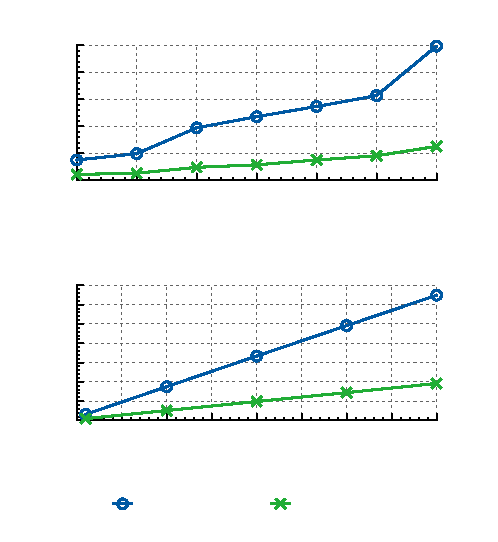
\includegraphics{plots/search}}%
    \gplfronttext
  \end{picture}%
\endgroup
